\documentclass[conference]{IEEEtran}
\IEEEoverridecommandlockouts
% The preceding line is only needed to identify funding in the first footnote. If that is unneeded, please comment it out.
\usepackage{cite}
\usepackage{amsmath,amssymb,amsfonts}
\usepackage{algorithmic}
\usepackage{graphicx}
\usepackage{textcomp}
\usepackage{xcolor}
\newcommand{\BibTeX}{\textrm{B \kern -.05em \textsc{i \kern -.025em b} \kern -.08em
T \kern -.1667em \lower .7ex \hbox{E} \kern -.125emX}}
\begin{document}

\title{The Efficacy of Chaotic Neural Networks for Asymmetric Encryption of Audio Files}

\author{\IEEEauthorblockN{1\textsuperscript{st} Patrick Pfenning}
\IEEEauthorblockA{\textit{School of Computing and Data Science} \\
\textit{Wentworth Institute of Technology}\\
Boston, MA \\
pfenningp@wit.edu}
}

\maketitle

\begin{abstract}
This document is a model and instructions for \LaTeX.
This and the IEEEtran.cls file define the components of your paper [title, text, heads, etc.]. *CRITICAL: Do Not Use Symbols, Special Characters, Footnotes, 
or Math in Paper Title or Abstract.
\end{abstract}

\begin{IEEEkeywords}
component, formatting, style, styling, insert
\end{IEEEkeywords}

\section{Introduction}\label{sec:introduction}

\subsection{History of Encryption}\label{subsec:history-of-encryption}

\subsection{Importance in Today's World}\label{subsec:importance-in-today's-world}

\section{Background}\label{sec:background}

\subsection{What is Chaos?}\label{subsec:what-is-chaos?}

\begin{itemize}
    \item Chaos is statistically indistinguishable from randomness~\cite{Alligood}
    \item Sensitivity to initial conditions
    \item Initial conditions used to build key
    \item \ldots
\end{itemize}

\subsection{Numeric Public-Key Algorithms}\label{subsec:numeric-public-key-algorithms}

\begin{itemize}
    \item RSA
    \item AES
    \item Triple DES
    \item Blowfish
    \item Twofish
    \item \ldots
\end{itemize}

\section{Literature Review}\label{sec:literature-review}~\cite{Lokesh,Hamdy,Gujral}



\section{Building the Network}\label{sec:building-the-network}

\subsection{Chaotic Functions}\label{subsec:chaotic-functions}

\begin{itemize}
    \item Hénon map
    \item Logistic map
    \item Lorenz system
    \item Tent map
    \item Horseshoe map
    \item \ldots
\end{itemize}

\subsection{Network and Diagram}\label{subsec:network-and-diagram}

Outline inputs and hidden layers here

\begin{figure}[!ht]
    \centering
    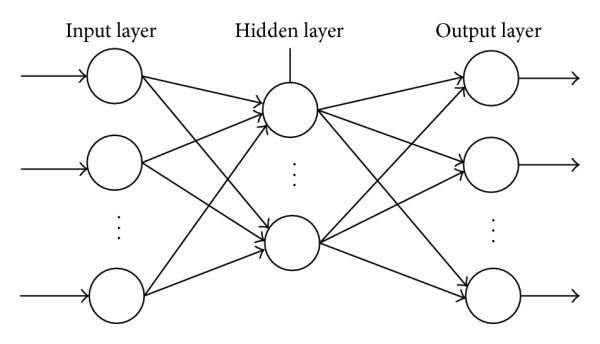
\includegraphics{figures/CNN}
    \caption{Example CNN Architecture}
    \label{fig:CNN}
\end{figure}

\section{Algorithm}\label{sec:algorithm}

\subsection{Key Generation}\label{subsec:key-generation}

\subsection{Diffusion}\label{subsec:diffusion}

\subsection{Encryption}\label{subsec:encryption}

\subsection{Decryption}\label{subsec:decryption}

\subsection{De-Diffusion}\label{subsec:de-diffusion}

\section{Experimentation and Results}\label{sec:experimentation-and-results}

Here we test our algorithm against several existing methods

\subsection{Processing Time and Complexity}\label{subsec:processing-time-and-complexity}

\subsection{Histogram Analysis}\label{subsec:histogram-analysis}

\subsection{Correlation Analysis}\label{subsec:correlation-analysis}

\subsection{Peak Signal to Noise Ratio}\label{subsec:peak-signal-to-noise-ratio}

\subsection{Encryption Quality}\label{subsec:encryption-quality}

\subsection{Vulnerability to Attacks}\label{subsec:vulnerability-to-attacks}

\subsection{Key Sensitivity}\label{subsec:key-sensitivity}

\section{Future Work}\label{sec:future-work}

\section{Conclusion}\label{sec:conclusion}

\section{Acknowledgments}\label{sec:acknowledgments}

\bibliographystyle{ieeetr}
\bibliography{bib/bibliography}

\end{document}
